
{\it Section prepared by the Working Group: 'Monte Carlo predictions for jet substructure', \underline{A. Arce}, D. Bjergaard, A. Buckley, M. Campanelli, \underline{D. Kar}, K. Nordstrom.
}



In order to use boosted objects and substructure techniques for measurements and
searches, it is important that Monte Carlo generators describe the jet
substructure with reasonable precision, and that
variations due to the choice of parton shower models and their
parameters are characterized and understood.  
We study jet mass, before and after several jet grooming procedures,
a number of popular jet substructure observables, colour flow and jet charge.
For each of these we compare the predictions of 
several parton shower and hadronisation codes, not only in 
\emph{signal-like} topologies, but also in
background or calibration samples.  

%{\em Marcel Vos: I assume W+jets is your background process. 
%The theory section proposes measurements in Z+jets. I guess it's rather late to amend this. 
%Could we argue that these are sufficiently similar? 
%\textbf{Ans: Please see the updated text. Yes, these processes are quite similar.  
%W+jets offers the advantage of allowing us to predict the leading jet's charge sign with about $70\%$ accuracy.} }


\subsection{Monte Carlo samples and tools}


Three processes in $pp$ collisions are considered
at $\sqrt{s}=7$~TeV: semileptonic \ttbar decays, boosted 
semileptonic \ttbar decays, and $(W^\pm \rightarrow \mu\nu)+$jets.
These processes provide massive jets coming from hadronic decays of a
colour-neutral boson as well as jets from heavy and light quarks. 

Like $Z$+jets, the  ($W\rightarrow \mu\nu)$+jets 
process provides a well-understood source of quarks and gluons, 
and additionally allows an experimentally accessible identification 
(``away-side-tag'') of the charge of the leading jet.  
Assuming that the charge of this jet is opposite to the muon's 
charge leads to the same charge assignment as a conventional parton matching scheme in approximately 70\% of simulated events in leading order Monte Carlo simulation; 
in the remaining 30\% of cases, the recoiling jet matches a (charge-neutral) gluon.

The selection of $t$, $W^\pm$, and quark 
jet candidates for the distributions compared below include event 
topologies that can be realistically collected in the 
LHC experiments, with typical background rejection cuts, so that these studies, 
based on simulation, could be reproduced using LHC data.

\begin{figure*}[t!]
  \centering 
   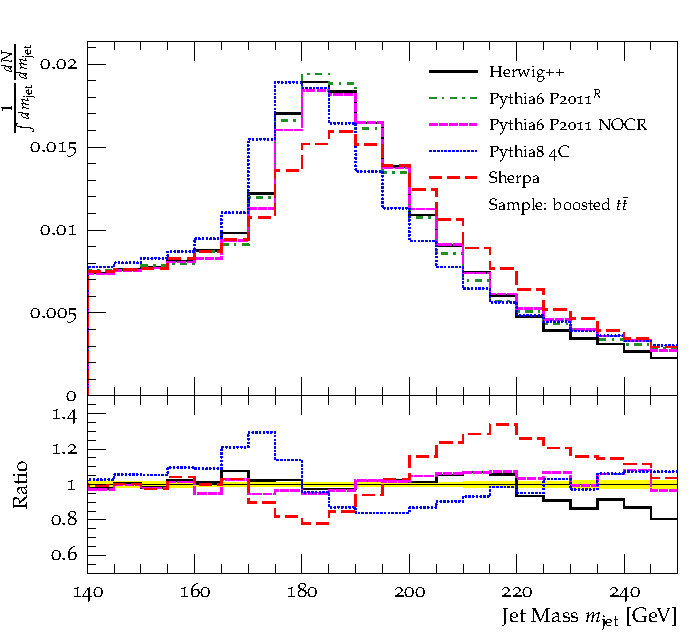
\includegraphics[width=0.42\textwidth]{MC_SUBSTRUCTURE_jetmass}
     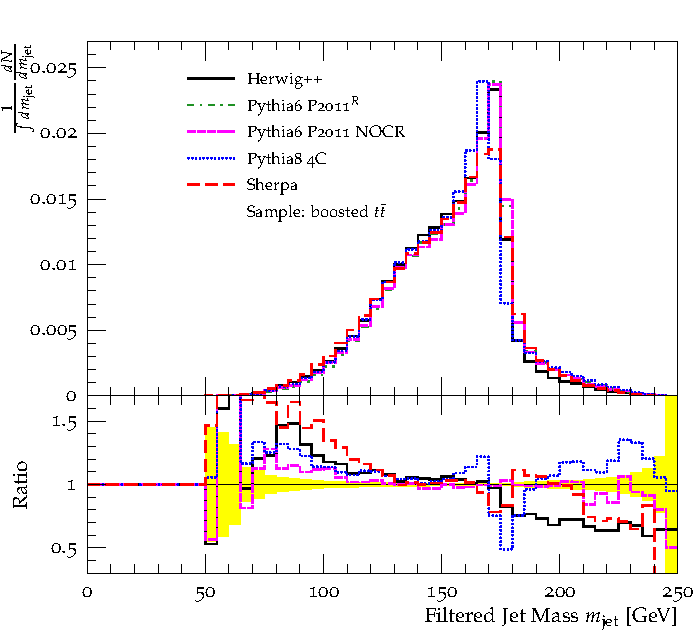
\includegraphics[width=0.42\textwidth]{MC_SUBSTRUCTURE_Filtered_mass} \\
     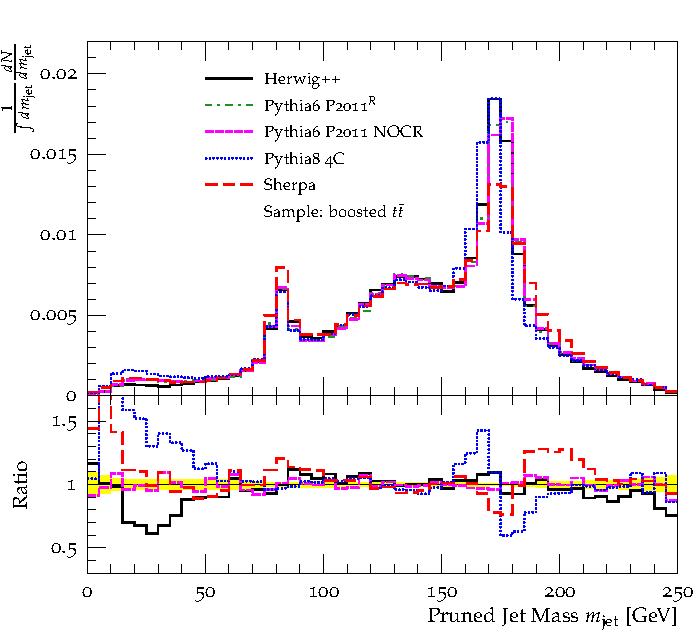
\includegraphics[width=0.42\textwidth]{MC_SUBSTRUCTURE_Pruned_mass}
      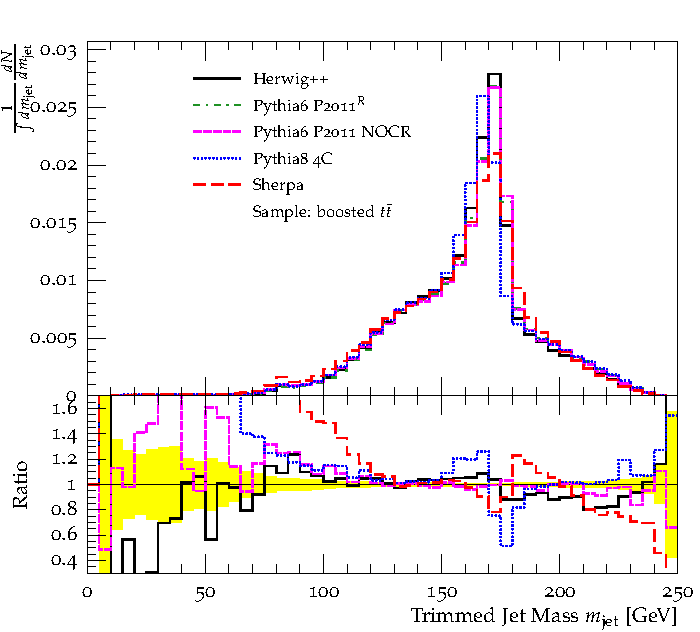
\includegraphics[width=0.42\textwidth]{MC_SUBSTRUCTURE_Trimmed_mass}
    \caption[]{
The jet invariant mass distribution for the leading  jet in the boosted 
semileptonic \ttbar{} event sample, before and after jet grooming.}
  \label{fig:jmass}
\end{figure*}

The most commonly used leading order (LO) Monte Carlo simulation codes are
the \textsc{Pythia} and \textsc{Herwig} families. 
Here, predictions from the Perugia 2011~\cite{Skands:2009zm} tune with
CTEQ5L~\cite{Lai:1999wy} parton density function (PDF) and corresponding 
NOCR tunes of \textsc{pythia6}~\cite{Sjostrand:2000wi,Sjostrand:2006za}
(version 6.426), tune 4C~\cite{Corke:2010yf} with CTEQ6L1 PDF~\cite{cteq6} 
of the newer \texttt{C++} \textsc{Pythia8} generator~\cite{Sjostrand:2007gs}
(version 8.170), and the LHC-UE-EE-4~\cite{Gieseke:2012ft} tune of
\hpp~\cite{Bahr:2008pv,Gieseke:2011na} (version 2.6.1) with CTEQ6L1 
PDF are compared. The default parameter tune of the
next-to-leading order (NLO) parton shower model implemented in
\textsc{Sherpa}~\cite{Gleisberg:2008ta} (version 1.4.2) with CT10 
PDF~\cite{Lai:2010vv} is also included in comparisons. 
The \textsc{Pythia6} generator with the Perugia2011 tune is taken as a 
reference in all comparisons. 
For each generator, tune and process 1 million proton-proton events at $\sqrt{s}=$ 7~\tev{} are produced.




The analysis relies on the FastJet 3.0.3 package~\cite{Cacciari:2011ma,Cacciari:2008gn} 
and Rivet analysis framework~\cite{Buckley:2010ar}. All 
analysis routines are available on the conference web page~\cite{rivetroutines}.
In the boosted semileptonic \ttbar analysis, 
large-radius jets were formed using the anti-$k_t$ 
algorithm~\cite{Cacciari:2008gp} with a radius parameter of $1.2$
using all stable particles within pseudorapidity $|\eta| < 4$.
The jets are selected if they passed 
the following cuts: $p_T^{\text{jet}} > 350$ GeV, 140 GeV
$ < m^{\text{jet}} < 250$ GeV. 
Only the leading and subleading jets were selected if more than two 
jets passed the cuts.
The subjets were formed using the Cambridge-Aachen 
algorithm~\cite{Dokshitzer:1997in,Wobisch:1998wt} with radius $0.3$.




\subsection{Jet mass}


The jet mass distribution for the leading jet in the boosted semi-leptonic
\ttbar{} sample is shown in Fig.~\ref{fig:jmass}. The  
parton shower models in \textsc{Pythia6}, \textsc{Pythia8}, \textsc{Herwig++} 
and \textsc{Sherpa} yield significantly different predictions. 
Important differences
are observed in the location and shape of the top quark mass peak.
The largest deviations of the normalized cross section 
in a given jet mass bin amount to approximately 20\%. 
Much better agreement is obtained for predictions with different tunes of a 
single generator.

The effect of different grooming techniques on jet mass is also shown in 
Fig.~\ref{fig:jmass}. For filtering, three hardest subjets with $R^{sub} =0.3$ are used.
The trimming uses all subjets over $3\%$ of $p_T^{jet}$ and $R^{sub} = 0.3$.
For pruning, $z = 0.1$ and $D = m^{jet} / p_T^{jet}$ is used.
As expected, a much narrower top quark mass peak 
is obtained, with a particularly strong reduction of the high-mass tail. 
The grooming procedure improves the agreement among the 
different Monte Carlo tools, as expected from previous Monte Carlo studies
with a more limited set of generators~\cite{Abdesselam:2010pt} and
comparison with data~\cite{ATLAS:2012am}. 
 




\begin{figure*}[t!]
  \centering
%\subfigure[angular structure function $r_{*n}$]{
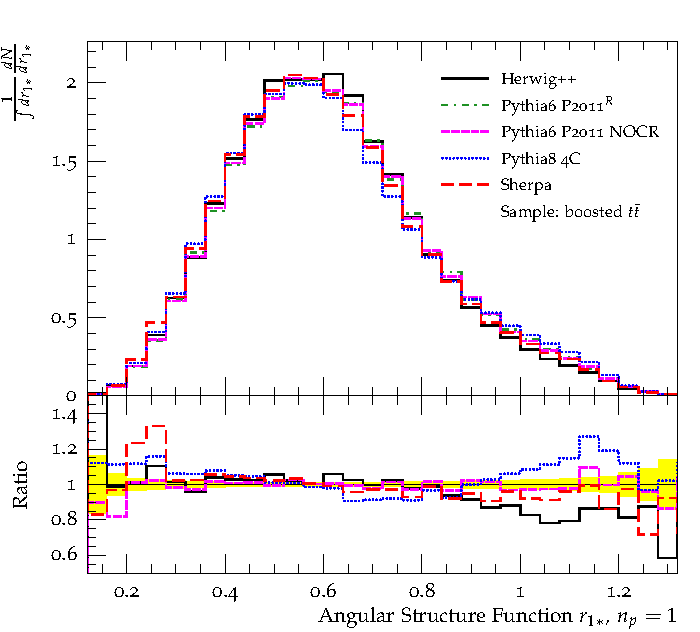
\includegraphics[width=0.42\textwidth]{MC_SUBSTRUCTURE_1_peak_r.pdf}
%\subfigure[n-subjettiness $\tau_{3/2}$]{
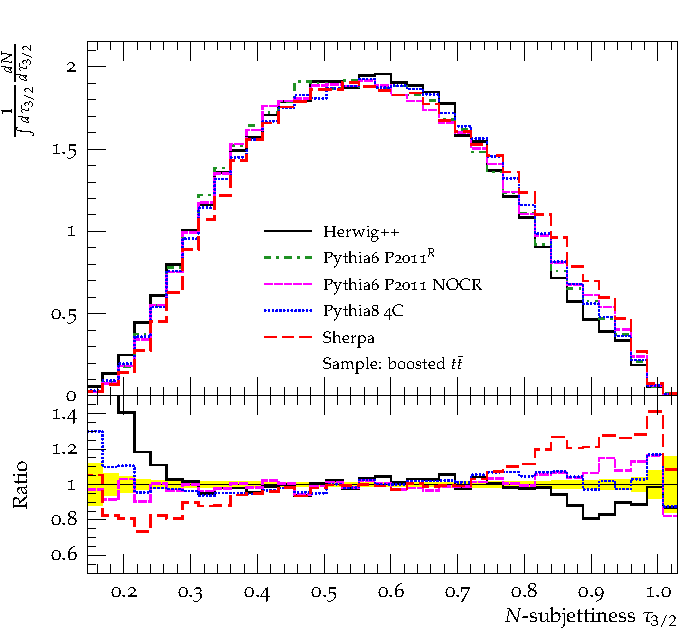
\includegraphics[width=0.42\textwidth]{MC_SUBSTRUCTURE_Tau_32.pdf} \\
%\subfigure[angularity $\tau_{-2}$]{
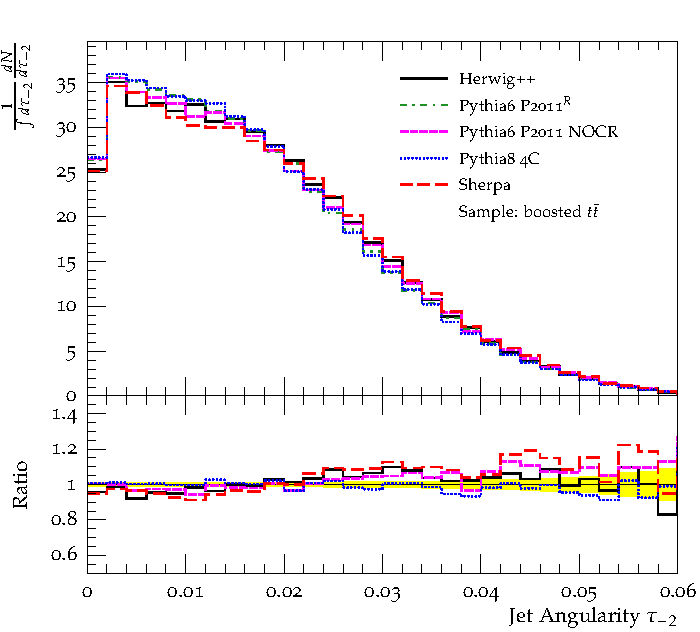
\includegraphics[width=0.42\textwidth]{MC_SUBSTRUCTURE_Angularity.pdf}
%\subfigure[eccentricity $\epsilon$]{
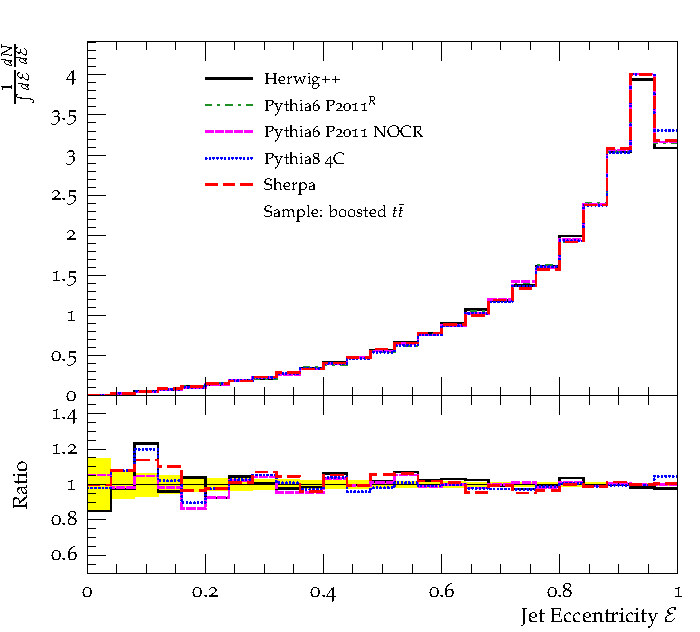
\includegraphics[width=0.42\textwidth]{MC_SUBSTRUCTURE_Eccentricity.pdf} \\
         \caption[]{The distribution 
         of four different measures of jet substructure
         for leading jet of a boosted semileptonic top sample. 
         The C-A algorithm is used in reclustering, as mentioned in the text.}
  \label{fig:substructureobservables}
\end{figure*}



\begin{figure*}[t!]
  \centering
%   \includegraphics[width=0.32\textwidth]{MC_GENSTUDY_JETCHARGE_JetPullTheta} 
     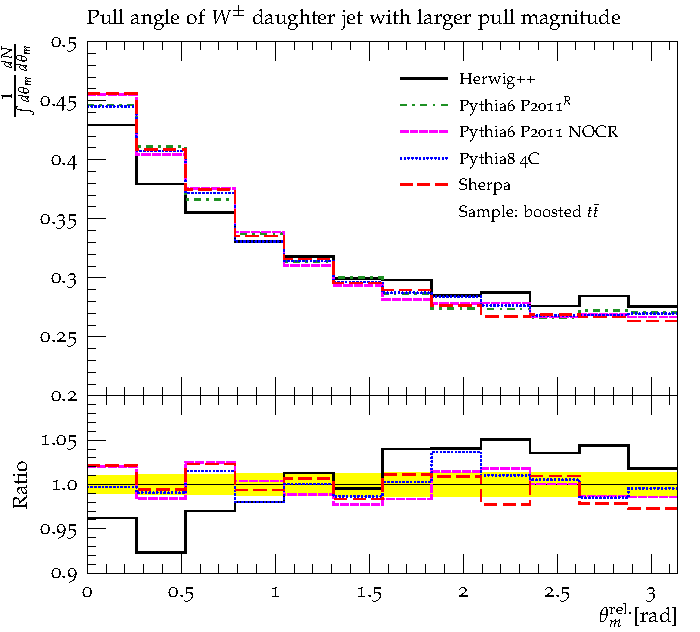
\includegraphics[width=0.42\textwidth]{MC_CFLOW_TOPBOOST_LargePullAngleToDipoleAxis} 
      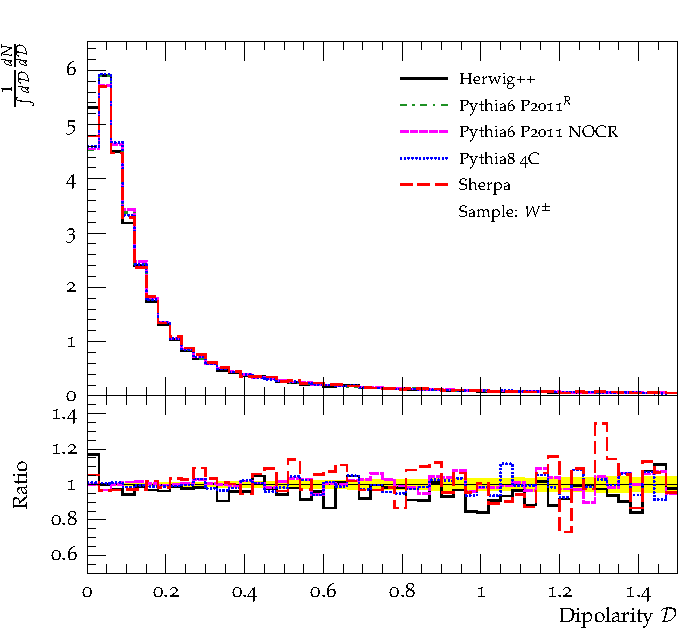
\includegraphics[width=0.42\textwidth]{MC_GENSTUDY_JETCHARGE_Dipolarity}
      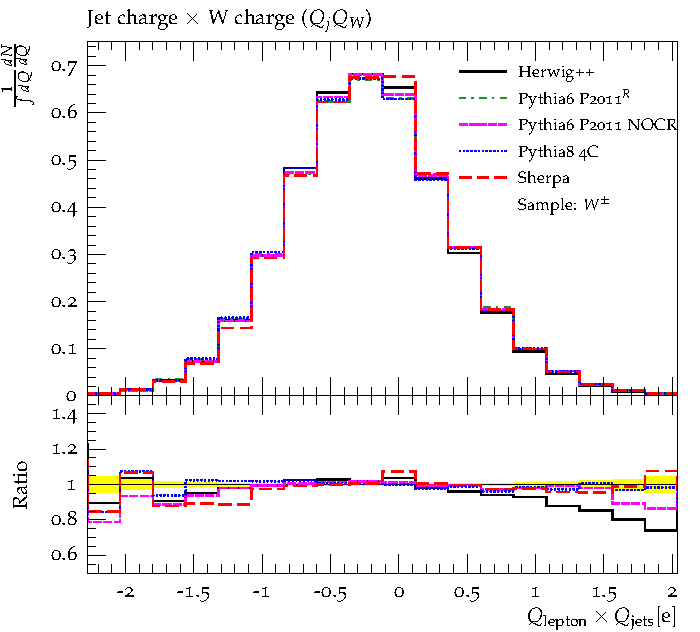
\includegraphics[width=0.42\textwidth]{MC_GENSTUDY_JETCHARGE_WJetChargeK3}%Fixme!
      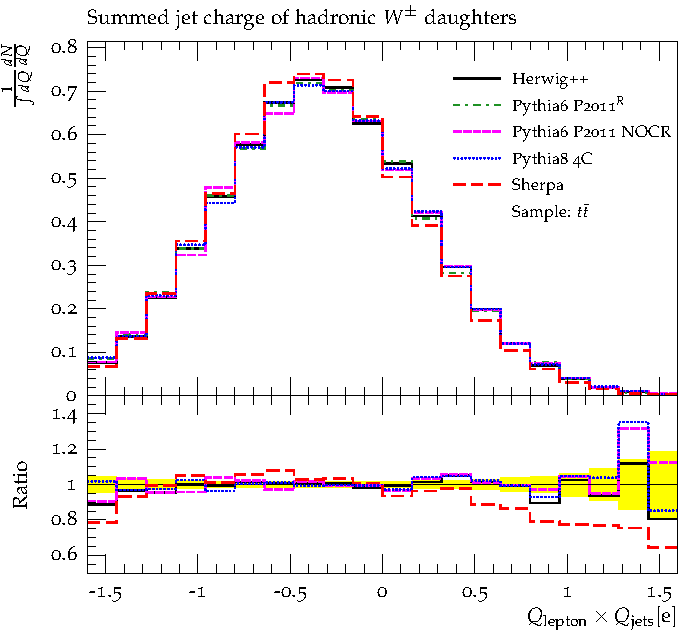
\includegraphics[width=0.42\textwidth]{MC_CFLOW_TTBAR_HadronicWJetChargeSum}
 \caption[]{
 Upper row: Comparison of colour-flow observables: pull angle of leading jet 
 attributed to the hadronic W decay in \ttbar{} events, and 
 dipolarity of leading jet produced in association with a leptonically decaying W.
 Lower row: Comparison of jet charge observables  ($\kappa=0.3$): 
 charge observable for leading jet produced in association with a 
 leptonically decaying W (left panel), and sum of jet charge observables for the 
 two jets attributed to the hadronic W  decay in \ttbar{} events (right panel).
}
  \label{fig:cflow}
\end{figure*}
%Description of Fig 1/2



\subsection{Jet substructure observables}
We investigate the spread among generators for a number of other 
substructure observables on the market:

\begin{itemize}


\item The Angular Correlation Function~\cite{Jankowiak:2011qa}
measures the $\Delta R$ scale of a jet's radiation. It is defined as:
\[ \mathcal{G}(R) = \frac{1}{\sum p_{T,i} p_{T,j} \Delta R_{i,j}^2} \sum p_{T,i} p_{T,j} \Delta R_{i,j}^2 \Theta(R - \Delta R_{i,j}) \]
where the sum runs over all pairs of particles in the jet, 
and $\Theta(x)$ is the Heaviside step function. 
The Angular Structure Function is defined as the following derivative:
\[ \Delta \mathcal{G}(R) = \frac{ d \hspace{0.1cm} \text{log} \hspace{0.1cm} \mathcal{G}(R) }{d \hspace{0.1cm}\text{log} \hspace{0.1cm} R} \]
Peaks in $\Delta \mathcal{G}(R)$~\footnote{
In this analysis the derivatives are smoothed using a 
Gaussian in the numerator and an error function in the denominator, both 
with $\sigma = 0.06$}
can then be found which 
correspond to $\Delta R$ scales with excess radiation in the jet. 
The variable $r_{1*}$ is the point in the $dR$-spectrum that the first peak in the angular structure 
function appears at,  and $n_p$ is the total number of peaks in the jet's angular structure function.
The prominence $h$ of the highest peak is 
defined as its height. The prominence of any lower peak 
is defined as the minimum vertical descent that is required in descending 
from that peak before ascending a higher, neighboring peak.
A prominence of $h > 4$ for peaks in the angular 
structure function is required and the partial mass and $\Delta R$ scale
of the most prominent peaks are retained.


\item $N$-subjettiness~\cite{Thaler:2010tr,Thaler:2011gf} measures how much 
of a jet's radiation is aligned along 
$N$ subjet axes in the $y - \phi$ plane. It is defined as:
\[ \tau_N = \frac{1}{\sum\limits_k p_{T,k} R_{\text{jet}}^\beta } \sum\limits_k p_{T,k} \hspace{0.1cm} \text{min}(\Delta R_{1,k}^\beta, \Delta R_{2_k}^\beta, ...) \]
where $\Delta R_{n,k}$ is the distance from $k$ to the $n$th subjet axis in the $y - \phi$ plane, 
$R_{\text{jet}}$ is the radius used for clustering the original jet, 
and $\beta$ is an angular weighting exponent\footnote{To improve the performance of $N$-subjettiness it is possible to use a k-means clustering 
algorithm to find (locally) optimal locations for the subjet axes. 
In this analysis  $\beta = 1$ is used to find the subjet axes by reclustering with the $k_t$ algorithm.
The $k$-means clustering algorithm is run once,  
as with this angular weighting exponent it finds a local minimum immediately. 
No attempt is made to find the global minimum.}.



\item Angularity~\cite{Berger:2003iw} introduces an adjustable parameter
$a$ that interpolates between the well-known event shapes thrust 
and jet broadening. Jet angularity is an IRC safe variable (for $a<$ 2) 
that can be used to separate multijet background from jets
containing boosted objects~\cite{Almeida:2008yp}.
It is defined as:
\[ \tau_a = \frac{1}{m_{jet}} \sum\limits_{i\in jets} \omega_i \sin ^a \theta_i (1 - \cos \theta_i)^{1-a}  \]
where $\omega_i$ is the energy of a constituent of the jet.


\item 
Eccentricity~\cite{Chekanov:2010vc} of jets is defined by 
$1-v_{\text{max}}/v_{\text{min}}$, 
where $v_{max}$ and $v_{min}$ are the maximum and minimum values
of the  variances of jet constituents along the principle and minor 
axes\footnote{Eccentricity is strongly correlated with the 
planar flow, and it is a measure of jet elongation ranging
from 0 for perfectly circularly symmetric jet shapes to 1 for 
infinitely elongated jet shapes. This is primarily useful for
identifying high $p_T$ merged jets.}.

\end{itemize}

Most models predict very similar behavior for angularity, eccentricity
and the $\Delta R$ scale of the peak in the $n_p=1$ bin for the angular structure function.
Deviations are typically below 10\% for these observables.
The harder jet mass distribution in \textsc{SHERPA} and the softer spectrum
in \textsc{Pythia8} are reflected in the edges of the $\tau_{3/2}$ 
distribution.






\subsection{Colour flow}


%% 

Colour flow observables offer a complimentary way to probe boosted event 
topologies. Pull~\cite{Gallicchio:2010sw} is a $p_T$-weighted vector in 
$\eta-\phi$ space that is constructed so as to point from a given jet to 
its colour-connected partner(s). The pull is measured with 
respect to the other $W^\pm$ daughter jet. 
The $W$-boson is selected kinematically in $4$-jet events with $2$ 
$b$-quarks, and flavors are labelled using the highest $p_T$ cone.
In Fig.~\ref{fig:cflow}, the top left plot 
shows this variable for a background-like distribution. 
The comparisons demonstrate 
that Herwig produces a different colour flow structure.
%there may be enough statistics (but possibly too much pileup) to see this effect in data.

Dipolarity~\cite{Hook:2011cq} can distinguish whether a pair of subjets arises
from a colour singlet source. In the top right plot of Fig.~\ref{fig:cflow}, 
the dipolarity predictions are seen to be similar for all models considered.


\subsection{Jet charge}

%Description of Figure 6
Jet charge~\cite{Feynman1978,Waalewijn2012,Krohn2012} is constructed 
in an attempt to associate a jet-based observable to the charge of the 
originating hard parton. The $p_T$-weighted jet charge
\[
Q_j = \frac{1}{{p_T}_j^\kappa}\sum_{i\in T} q_i\times (p_T^i)^\kappa \]
is shown with $\kappa=0.3$ in Fig.~\ref{fig:cflow}, using anti-kt $0.6$ jets.
The comparison displays the most relevant distributions for typical quark tagging and boson tagging analyses.
Different MC models are seen to have very similar predictions for this observable too.

\subsection{Summary}


We have prepared the Rivet routines to evaluate the predictions of 
Monte Carlo generators for the internal structure of large 
area jets. The normalized predictions from several mainstream
Monte Carlo models are compared. Several aspects of jet substructure 
are evaluated, from basic jet invariant mass to colour flow observables 
and jet charge.

We find that for jet mass large variations are observed 
between the various MC models. 
However, for groomed jets the deviations between different model predictions 
are smaller. The differences between several recent tunes of the 
\textsc{Pythia} generator are much smaller.
The MC model predictions are similar for $N$-subjettiness, angularity 
and eccentricity. The \hpp model gives different predictions than other models 
for colour flow observables, but since the implementation of colour 
connection in \hpp model is very recent, this may lead to improvement 
of the model.


